\documentclass[10 pt]{article}
\usepackage{tikz}
\usetikzlibrary{arrows}
\usepackage[margin=0.5 in]{geometry}
\usepackage[utf8]{inputenc}
\usepackage{tabu}
\usepackage{color}
\usepackage{mathtools}

\usepackage{xcolor}
\usepackage{listings}
\usepackage{enumitem}
\usepackage{multicol}
\setlength{\columnsep}{1cm} 
\newtheorem{theorem}{Teorema}
\usepackage{mathrsfs}
\title{\textbf {Estructuras de Datos 1 - ST0245\\Segundo Parcial Grupo 033}}
\author{Nombre ..............................\\
		Departamento de Informática y Sistemas\\
		Universidad EAFIT\\}
\date{Mayo 14 de 2020}
\begin{document}
\lstdefinestyle{customc}{
	language=Java, 
	numbers=left, 
	showspaces=false,
    showstringspaces=false, 
    tabsize=2, 
    breaklines=true,
    xleftmargin=5.0ex,
}
\lstset{escapechar=@,style=customc, numbers=left, stepnumber = 1} 
\maketitle
\begin{multicols}{2}
\section{Pilas 20\%}

Cuando se realiza una obra de construcción, existen varios impactos ambientales que pueden ser medidos con indicadores de sostenibilidad. Un problema consiste en encontrar la combinación de procesos que minimizan estos tres indicadores de sostenibilidad: Las emisiones de $CO_2$, la energía consumida y los costos económicos. Este problema de optimización es un problema de búsqueda; por eso necesitamos que 
implementes el algoritmo \emph{búsqueda del primero en profundidad (DFS)} usando pilas. Como una ayuda se te entrega el siguiente código, al cual le faltan algunas líneas; por favor, complételas. ¡Vamos por el medio ambiente!

{\small
\begin{lstlisting}
void dfs(ArrayList<Integer>[] g, int v, boolean[] seen){
  Stack<Integer> s = new Stack();
  s.push(v);
  while(!s.empty()){
    v = ................;
    if(seen[v])
      .................
    seen[v] = true;
    for(int i=0; i<g[v].size(); ++i){
      int u = ..............;
      if(!seen[u])
        ..................;
} } }
\end{lstlisting}
}
\begin{enumerate}[label=\Alph*]
	% Respuesta: s.pop()
	\item (10\%) Completa la línea 5 ............................... \\
	% Respuesta: continue
	\ \ \ \ \ \ \ \ \ \ \ \ Completa la línea 7 ...............................
	% Respuesta: g[v].get(i)
	\item (10\%) Completa la línea 10 ............................... \\
	% Respuesta: s.push(u)
	\ \ \ \ \ \ \ \ \ \ \ \ Completa la línea 12 ...............................
\end{enumerate}

Pista: La palabra reservada \texttt{continue} se salta la iteración actual un ciclo y salta a la siguiente; la palabra \texttt{break} termina abruptamente un ciclo. En una pila, el método \texttt{push} ingresa un elemento a la pila y \texttt{pop} lo returna y elimina.

\section{Colas 20\%}
En el curso de Organización de Computadores (obligatoria para Sistemas, electiva para Matemáticas), profundizaremos sobre el uso de números binarios en la definición de las operaciones que realiza la unidad central de procesamiento (CPU). Mientras tanto, resolvamos el siguiente problema: 
Dado un entero $N$, genera los binarios entre $1$ y $N$. Por ejemplo, si $N = 7$, entonces la respuesta es $[1, 10, 11, 100, 101, 111]$. El siguiente código, resuelve el problema, pero faltan algunas líneas; por favor, complételas.
{\small
\begin{lstlisting}
List<String> solve(int N){
  List<String> res = new ArrayList();
  Queue<String> q = new ArrayDeque();
  q.add("1");
  for(int i = 0; i < N; ++i){
    q.add(........... + "0");
    q.add(........... + "1");
    res.add(q.poll());
  }
  return res;
}
\end{lstlisting}
}
\begin{enumerate}[label=\Alph*]
	% Respuesta: O(n) o O(N)
	\item (10\%) ¿Cuál es la complejidad asíntotica, en el peor de los casos, del algoritmo anterior? ........................................
	% Respuesta: q.peek()
	\item (10\%) Completa la línea 6 ........................................
	% Respuesta: q.peek()
  \ \ \ \ \ \ \ \ \ \ \ \ \ \ Completa la línea 7 ........................................
\end{enumerate}

\emph{ArrayQueue} es una clase que implementa una cola con arreglos. El método \texttt{poll} elimina y retorna un elemento de la cola, \texttt{peek} permite verlo sin eliminarlo y \texttt{add} ingresa un elemento a la cola.

\section{Tablas de Hash 20\%}
Cuando un sitio web te solicita tu login y password para autenticarte, el password que se almacena en el servidor es el el hash del password. De esa manera, si un atacante accede a los passwords almacenados en el servidor, estos no le serán útiles para autenticarse en el sitio web. 
Para el siguiente ejercicio, se usa la función de hash \\$hash(s) = \sum\limits_{i = 0}^{|s| - 1} s[i] * p^i \mod m$, donde $p$ es un número primo menor que $40$,  $m$ es $10^9 + 7$ y $mod$ es el módulo (o residuo) de la división entera. 

Te entregan $n$ cadenas de caracteres de tamaño no mayor que $m$. La idea es encontrar cuantas de esas cadenas de caracteres son diferentes. Por ejemplo, si la entrada es $s = ["aba", "abc", "abcd", "aba", "aba", "abd", "abb", "abcd"]$, entonces la respuesta es $5$. El siguiente código resuelve el problema, pero faltan algunas líneas; por favor, complételas.

{\small
\begin{lstlisting}
int solve(String[] s){
  long[] h = new long[s.length];
  for(int i = 0; i < s.length; ++i){
    h[i] = hash(s); 
  }
  Arrays.sort(h); // Sort es O(n. log n)
  int cnt = 0;
  for(int i = 0; i < s.length; ++i){
    if(..................)
      cnt ++;
  }
  return cnt;
}
\end{lstlisting}
}
\begin{enumerate}[label=\Alph*]
	% Respuesta: O(nm + n log n)
	\item (10\%) En términos de $n$ y de $m$, ¿cuál es la complejidad asintótica, en el peor de los casos, del algoritmo anterior? .................................
	% Respuesta: i == 0 || h[i] != h[i - 1]
	\item (10\%) Completa la línea 9 .................................
\end{enumerate}

Pista: No olvides la complejidad de \texttt{hash(s)}

\section{Árboles 30\%}
El árbol de codificación de Huffman es un tipo de árbol binario que se utiliza para compresión de datos sin pérdidas en formatos como mp3 y jpg. Volviendo a los temas del curso, en este problema,
como bien sabes, un \emph{árbol} es un grafo no dirigido con $n$ vértices y $n - 1$ artistas; también se puede asumir que el peso de cada arista es de 1. Considera un árbol con raíz en el nodo $v$, sabemos que $d_i$ (usando el algoritmo de \emph{búsqueda primero en amplitud} [BFS] ) es la distancia mas corta desde el nodo $v$ al nodo $i$. En este ejercicio, vamos a encontrar el \textit{diámetro} de un árbol de $n$ nodos. El diámetro de un árbol se define como el largo máximo (es decir, el número de aristas) entre los caminos más cortos que hay entre cualesquiera dos vértices del árbol. En el siguiente árbol se describe su diámetro con una línea repintada, el cual es de $4$.
	\\
\begin{center}
	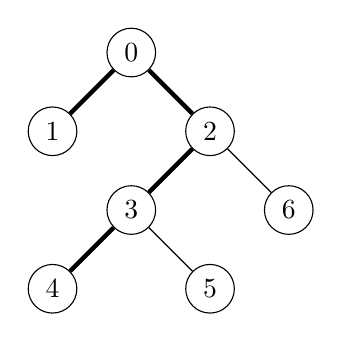
\begin{tikzpicture}	
	\tikzset{vertex/.style = {shape=circle,draw,minimum size=1.5em}}
	\tikzset{edge/.style = {-,> = latex'}}
	\node[vertex] (0) at (0, 0)  {0};
	\node[vertex] (1) at (-1, -1) {1};
	\node[vertex] (2) at (1, -1) {2};
	\node[vertex] (3) at (0, -2) {3};
	\node[vertex] (4) at (-1, -3) {4};
	\node[vertex] (5) at (1, -3) {5};
	\node[vertex] (6) at (2, -2) {6};
	%edges
	\draw[-, ultra thick] (0) to (1);
	\draw[-, ultra thick] (0) to (2);
	\draw[-, ultra thick] (2) to (3);
	\draw[-, ultra thick] (3) to (4);
	\draw[edge] (3) to (5);
	\draw[edge] (2) to (6);
	\end{tikzpicture}
\end{center}
El siguiente código encuentra el diámetro de un árbol, pero faltan algunas líneas; por favor, complétalas.

{\small
\begin{lstlisting}
int[] bfs(ArrayList<Integer>[] g, int v){
  int[] d = new int[g.length];
  Arrays.fill(d, Integer.MAX_VALUE);
  d[v] = 0;
  Queue<Integer> q;
  q = new LinkedList<Integer>();
  q.add(v);
  while(!q.isEmpty()){
    int s = q.poll();
    Iterator<Integer> i=g[s].listIterator();
    while(i.hasNext()){
      int n = i.next();
      if(d[s] + 1 < d[n]){
        d[n] = d[s] + 1;
        q.add(n);
  } } }
  return d;
}
int diametro(ArrayList<Integer> g[]){
  int v, u, w;
  v = u = w = 0;
  int[] d = bfs(g, v);
  int n = d.length;
  for(int i = 0; i < n; ++i)
    if( ............ ) u = i;
    int[] f = bfs(g, u);
    for(int i = 0; i < n; ++i)
      if( .......... ) w = i;
  return f[w];
}
\end{lstlisting}
}

El método \texttt{Arrays.fill(a,v)} coloca el valor $v$ en todas las posiciones del arreglo $a$.

\begin{enumerate}[label=\Alph*]
	% Respuesta: d[i] > d[u]
	\item (10\%) Completa la línea 25 ..........................
  \begin{enumerate}
    \item $d[u] > d[i]$
    \item $d[i] > d[u]$
    \item $f[w] > f[i]$
    \item $f[i] > f[w]$
  \end{enumerate}  
	% Respuesta: f[i] > f[w]
 \item (10\%) Completa la línea 28 ..........................
 \begin{enumerate}
    \item $d[u] > d[i]$
    \item $d[i] > d[u]$
    \item $f[w] > f[i]$
    \item $f[i] > f[w]$
  \end{enumerate}  

	% Respuesta: O(n)
	\item (10\%) ¿Cuál es la complejidad asintótica, en el peor de los casos, del algoritmo anterior? .................................
\end{enumerate}



\section{Grafos 10\%}
En la vida real, un grafo se utiliza para representar los mapas de \emph{Google Maps}. 
Para cada una de las siguiente proposiciones, determine si son verdaderas o falsas.
\begin{enumerate}[label=\Alph*]
  \item (10\%) Al representar un grafo completo con matrices de adyacencia y con listas de adyacencia, en ambos casos, el consumo de memoria (NO tiempo, sino memoria) es $O(n)$.
  \begin{enumerate}
    % Respuesta: Falso
    \item Verdadero
    \item Falso
  \end{enumerate}
  Cuando representamos un grafo con matrices de adyacencia, la complejidad asintótica, en el peor de los casos, de insertar un nuevo vértice es $O(n^2)$,  donde $n$ es el número de vértices.
  \begin{enumerate}
    % Respuesta: Verdadero
    \item Verdadero
    \item Falso
  \end{enumerate}
\end{enumerate}

Un grafo completo es áquel donde existe una arista entre cada par de vértices del grafo. 


\end{multicols}
\end{document}